\subsection{Power Play: Antenna Gains Unleashed!}

\begin{tcolorbox}[colback=gray!10, colframe=black, title=E9B07] What is the difference in radiated power between a lossless antenna with gain and an isotropic radiator driven by the same power?

\begin{enumerate}[label=\Alph*]
    \item The power radiated from the directional antenna is increased by the gain of the antenna.
    \item The power radiated from the directional antenna is stronger by its front-to-back ratio.
    \item \textbf{They are the same.}
    \item The power radiated from the isotropic radiator is 2.15 dB greater than that from the directional antenna.
\end{enumerate} \end{tcolorbox}

In this question, we explore the relationship between the power radiated by a lossless antenna with gain and an isotropic radiator when they are both driven by the same input power. To comprehend the answer, it is vital to understand a few key concepts:

\subsubsection{Antenna Types}
1. \textbf{Isotropic Radiator::} This is a hypothetical antenna that radiates power uniformly in all directions. It serves as a reference point for comparing other antennas.
2. \textbf{Directional Antenna::} This type has gain, meaning that it radiates more power in certain directions rather than uniformly like an isotropic radiator. The gain typically is expressed in decibels (dBi) relative to an isotropic radiator.

\subsubsection{Antenna Gain}
The gain of an antenna does not change the total power supplied to it but instead alters how power is distributed in different directions. For example, if we have a directional antenna with a gain of, say, 3 dB, this indicates that the power is concentrated more in one direction compared to isotropic radiation, but the total power radiated remains the same when considered over the whole sphere. 

\subsubsection{Understanding Power Radiated}
If both the directional antenna and the isotropic radiator are fed with the same input power, then, regardless of the gain of the directional antenna, the total power radiated by both remains equivalent when averaged over all directions. Hence, for a lossless antenna with gain, the power radiated does not exceed the total input power—it simply redistributes the power.

\subsubsection{Conclusion}
Given these definitions and concepts, the correct answer to the question posed is indeed:

\textbf{C: They are the same.}

This conclusion applies under ideal conditions with a lossless antenna and the same power input in both cases. Any additional gain mechanisms, such as antennas with front-to-back ratios, do not directly affect the total radiated power relative to an isotropic source. 

\subsubsection{Diagram}
The following diagram illustrates the concept theoretically, showing the isotropic radiator and a directional antenna with gain distributing power within their radiation patterns.

\begin{center}
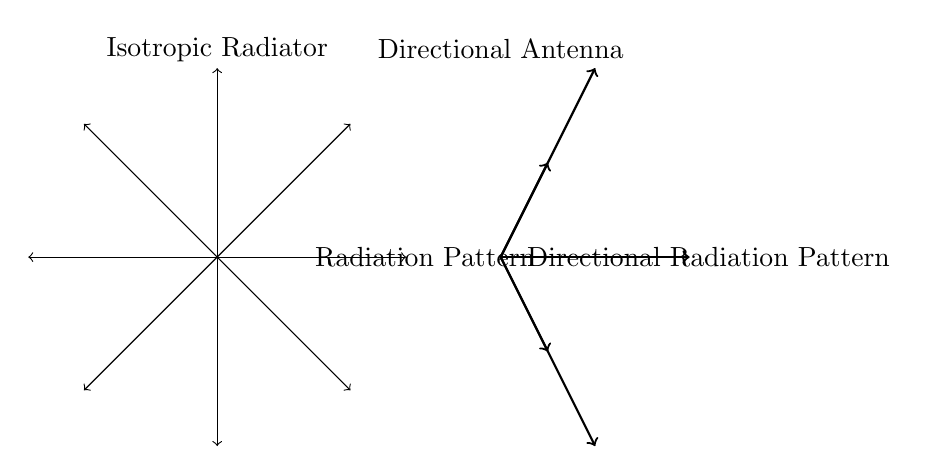
\begin{tikzpicture}[scale=1.2]
    % Isotropic radiator
    \draw[->] (0,0) -- (2,0);
    \draw[->] (0,0) -- (0,2);
    \draw[->] (0,0) -- (-2,0);
    \draw[->] (0,0) -- (0,-2);
    \draw[->] (0,0) -- (1.41,1.41);
    \draw[->] (0,0) -- (-1.41,1.41);
    \draw[->] (0,0) -- (-1.41,-1.41);
    \draw[->] (0,0) -- (1.41,-1.41);
    
    % Labels
    \node at (0,2.2) {Isotropic Radiator};
    \node at (2.2,0) {Radiation Pattern};
    
    % Directional antenna
    \draw[thick,->] (3,0) -- (5,0);
    \draw[thick,->] (3,0) -- (4,2);
    \draw[thick,->] (3,0) -- (4,-2);
    \draw[thick,->] (3,0) -- (3.5,1);
    \draw[thick,->] (3,0) -- (3.5,-1);
    
    \node at (3,2.2) {Directional Antenna};
    \node at (5.2,0) {Directional Radiation Pattern};
\end{tikzpicture}
\end{center}